\documentclass[11pt,spanish]{article}
\usepackage{selinput}
\usepackage[T1]{fontenc}
\usepackage{graphicx}
\usepackage{xcolor}

\usepackage[spanish]{babel}

%
\usepackage{tikz}
\usepackage{calc}
\usepackage{booktabs}
%\usepackage{hyperref}

% colors
\definecolor{color1}{HTML}{009FC7}
%\definecolor{color1}{HTML}{8C260F}
\definecolor{color2}{HTML}{333333}


% fonts
\usepackage{fontspec}
\defaultfontfeatures{Mapping=tex-text}
\setmainfont
[BoldFont=Lato-Bold.ttf,
ItalicFont=Lato-Italic.ttf,
BoldItalicFont=Lato-BoldItalic.ttf]
{Lato-Regular.ttf}
\newfontfamily\headingfont[ItalicFont=Lato-BlackItalic.ttf]{Lato-Black.ttf}
%%%

\usepackage{geometry}
\geometry{a4paper,
hmargin=20mm,vmargin=20mm,
head=0ex,foot=3ex}

\linespread{1.3}

\usepackage[hang]{caption}
\DeclareCaptionFormat{upper}{#1#2\uppercase{#3}\par}
\captionsetup{labelfont={bf,color=color2},textfont={normalsize,color=color2},format = upper,figurename=FIGURE,tablename=TABLE}

%%% fancy sections
\usepackage{titlesec}
\titleformat{\chapter}{\headingfont\LARGE\bfseries\scshape\color{color1}}{\thechapter}{1em}{}[\titlerule]
\titleformat{\section}{\color{color1}\headingfont\Large\bfseries\uppercase}{\thesection}{1em}{}[\titlerule]
\titleformat{\subsection}{\color{color1}\headingfont\large\bfseries\uppercase}{\thesubsection}{1em}{}
\titleformat{\subsubsection}{\color{color1}\headingfont\bfseries\uppercase}{\thesubsubsection}{1em}{}
%%%

% head and foot
\usepackage{fancyhdr}
\pagestyle{fancy}
\lhead{}
\chead{}
\makeatletter
\makeatother
\newlength{\myheight}
\lfoot{
\settoheight{\myheight}{\thepage}
\raisebox{-2ex-0.5\myheight}{
\includegraphics[height=4ex]{img/logo}}
}
\cfoot{\color{color2}Bandas Manager: Sistema para gestión de agrupaciones musicales}
\rfoot{\color{color2}\thepage}
\renewcommand\headrulewidth{0pt}
\renewcommand\footrulewidth{0pt}

%%% picture on cover page
\usepackage{eso-pic}
\newcommand\BackgroundPic{%
\put(0,0){%
\parbox[b][\paperheight]{\paperwidth}{%
\vfill
\centering
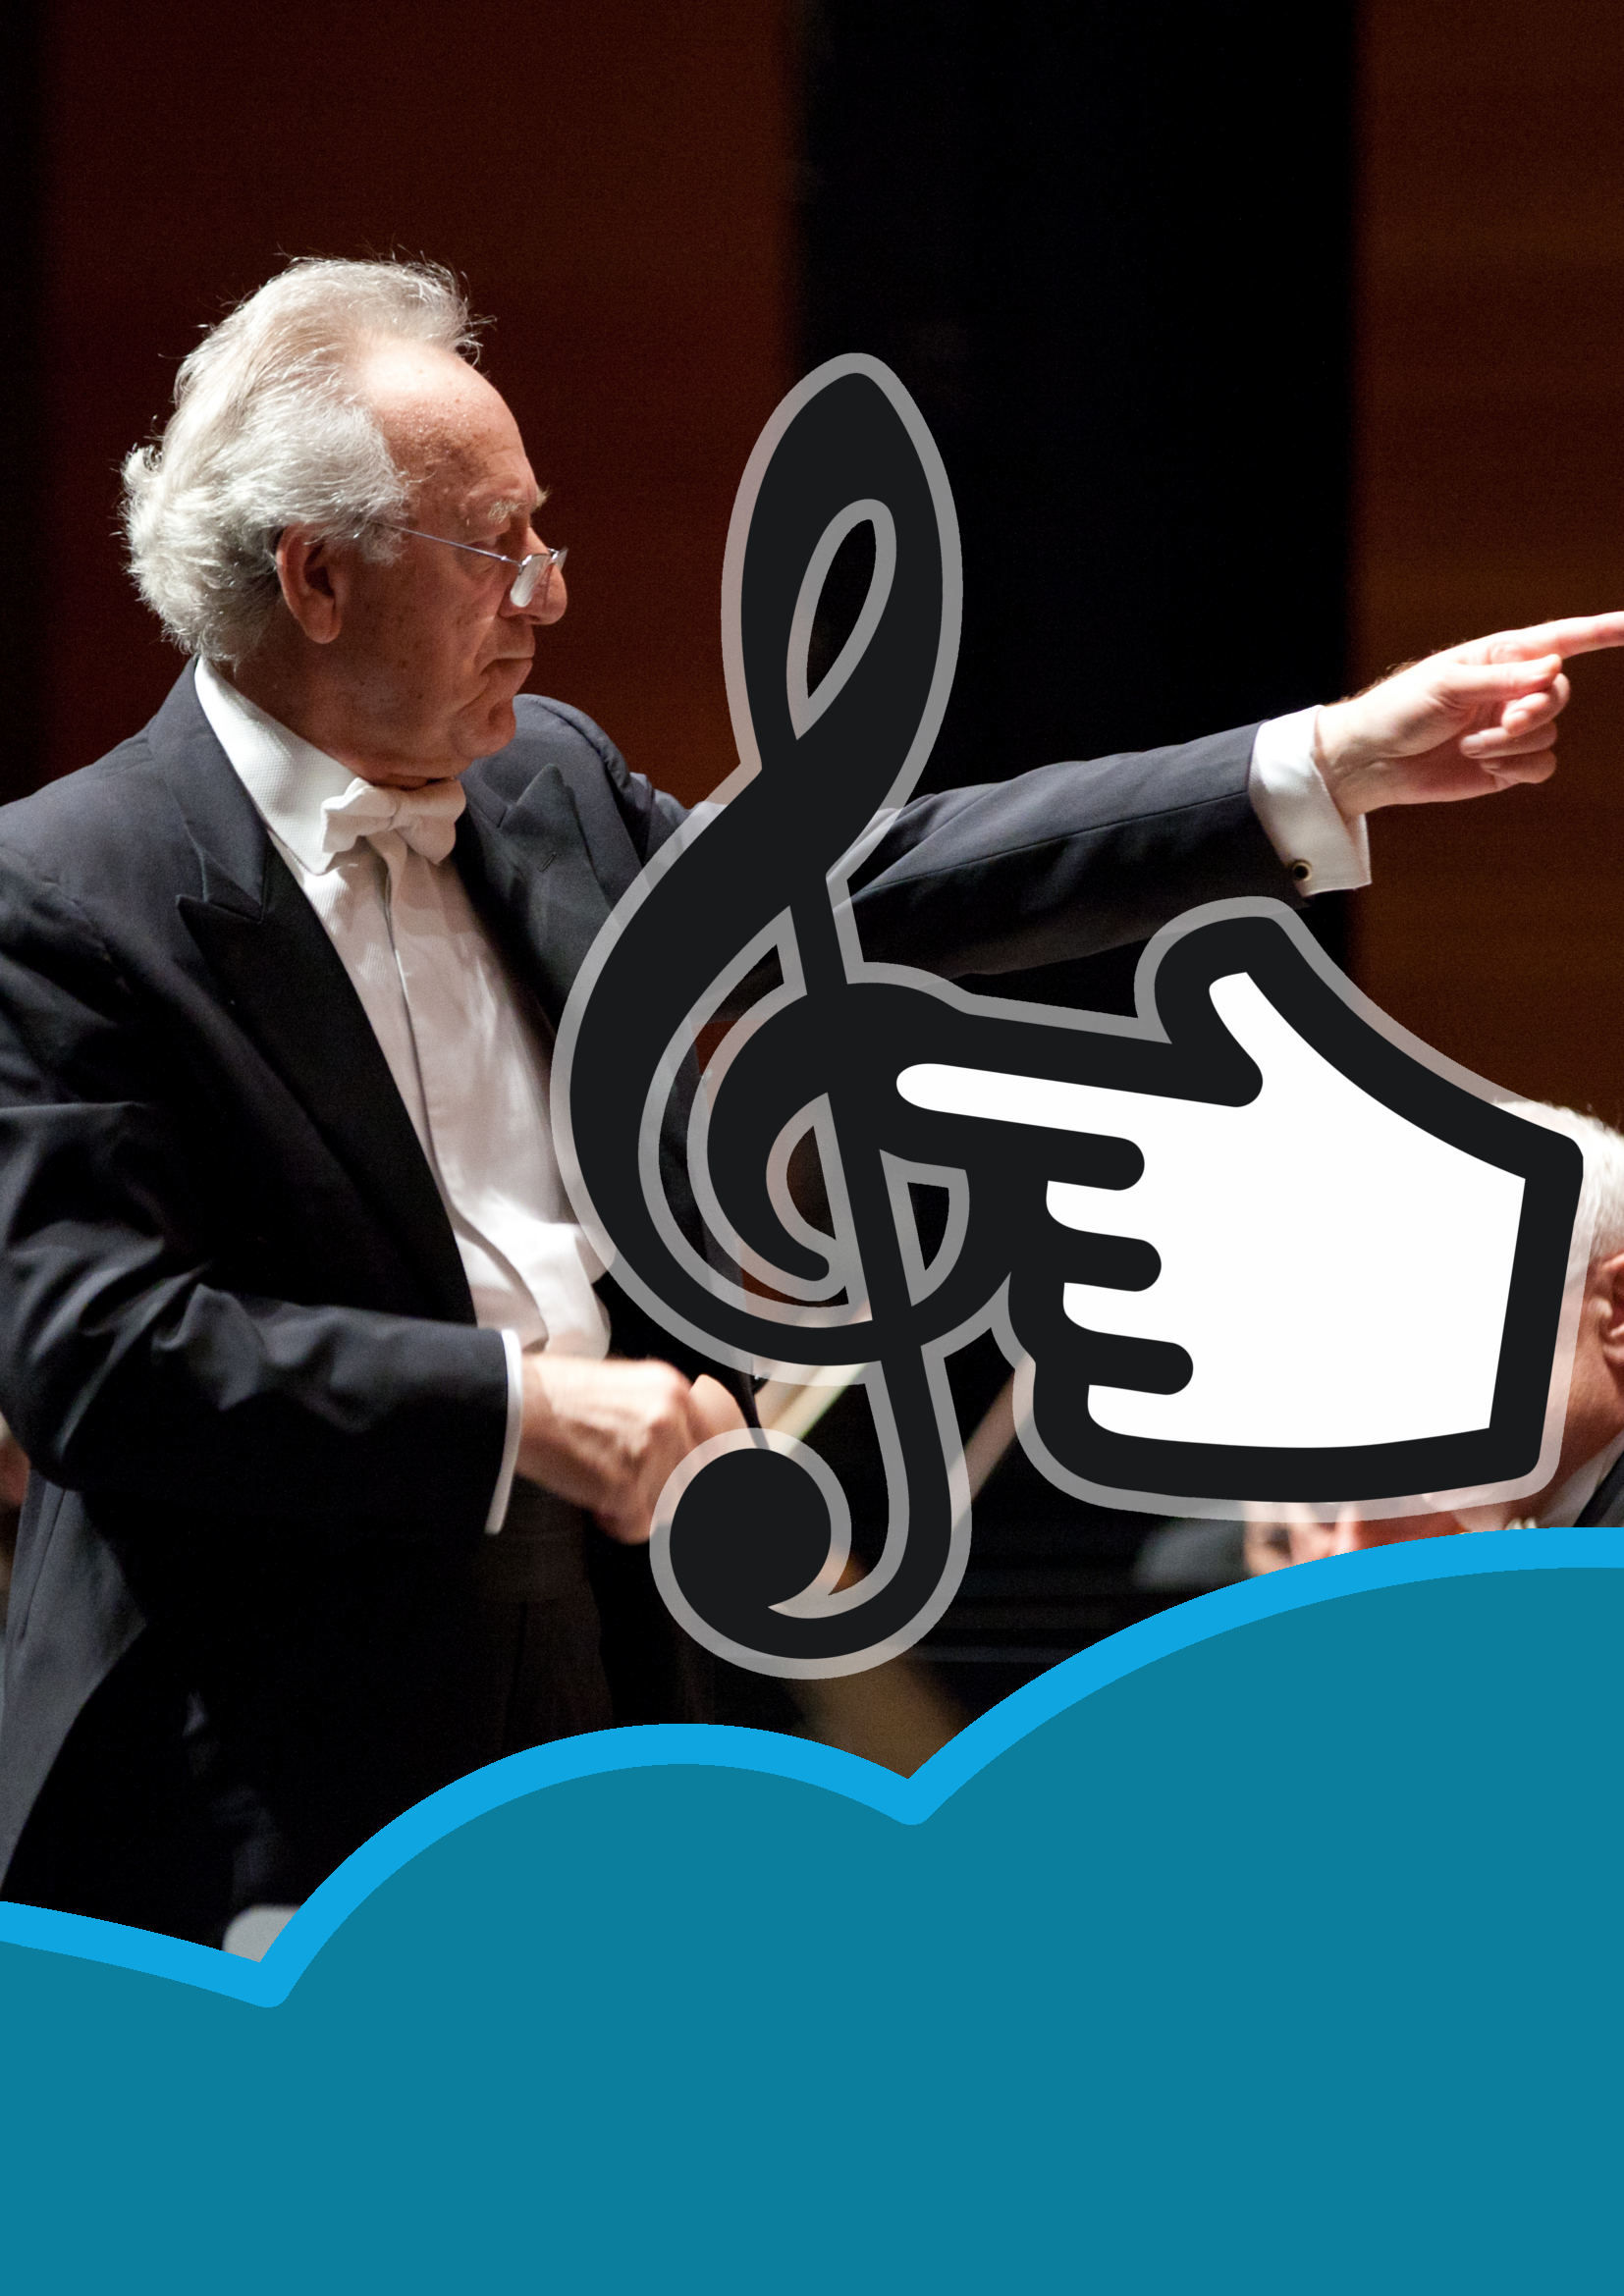
\includegraphics[width=\paperwidth,height=\paperheight,%
keepaspectratio]{cover}%
\vfill
}}}
%%%
% custom titlepage
\makeatletter
\renewcommand{\maketitle}{
\thispagestyle{empty}
\AddToShipoutPicture*{\BackgroundPic}
\ClearShipoutPicture
%
\phantom{a}
\vfill
\phantom{a}\hfill
\begin{tabular}[c]{@{}p{0.7\textwidth}@{}}
      \color{white}\headingfont\LARGE\@title\\[1em]
      \color{white}\headingfont\Large\@author\\[2em]
\end{tabular}
%
\clearpage
}
\makeatother
%%%


%%% fancy boxes
\usepackage{tcolorbox}
\usepackage{wrapfig}
\def\fullboxbegin{
\bigskip
\begin{tcolorbox}[colback=color1,colframe=color1,coltext=white,arc=0mm,boxrule=0pt]
}
\def\fullboxend{\end{tcolorbox}\medskip}
%
\def\leftboxbegin{
\begin{wrapfigure}{l}{0.5\textwidth}
\begin{tcolorbox}[colback=color1,colframe=color1,coltext=white,arc=0mm,boxrule=0pt]
}
\def\leftboxend{
\end{tcolorbox}
\end{wrapfigure}
}
%
\def\rightboxbegin{
\begin{wrapfigure}{r}{0.5\textwidth}
\begin{tcolorbox}[colback=color1,colframe=color1,coltext=white,arc=0mm,boxrule=0pt]
}
\def\rightboxend{
\end{tcolorbox}
\end{wrapfigure}
}
%
\newcounter{frames}
\def\frameboxbegin#1{
\bigskip
\refstepcounter{frames}
\begin{tcolorbox}[colback=white,colframe=color1,arc=0mm,title={\MakeUppercase{\textbf{Frame \arabic{frames}}: #1}}]
}
\def\frameboxend{
\end{tcolorbox}
}
%%%


\usepackage{lipsum}

%%%%%%%%%%%%%%%
% Title Page
\title{Band Manager}
\author{Sistema para gestión de agrupaciones musicales
        \newline / Israel Blancas}
%%%%%%%%%%%%%%%

\begin{document}
\maketitle

\tableofcontents
\clearpage

\section{Introducción}

\subsection{Breve estado del arte}

\noindent
Las bandas de música, orquestas y otros colectivos musicales, son grupos
formados por cierta cantidad de personas. Cuando el número de componentes es reducido,
la gestión de los mismos es relativamente sencilla pero, al aumentar el número de estos,
la situación puede volverse bastante complicada: la gestión de material, del patrimonio
musical, de material (tal como instrumentos o uniformes),
pasar lista, comunicaciones entre la junta directiva o el director con los componentes...


\subsection{Problemática}
Estos problemas se tratan de solventar mediante diversos sistemas:
\begin{itemize}
  \item \textbf{Comunicación director-componentes:} gracias a que el sistema de mensajería
  \textit{WhatsApp} insertó la opción de crear grupos o difusiones, la comunicación entre
  los miembros de la agrupación se ha facilitado. Por contra, si algún componente no
  desea facilitar a sus compañeros su número de teléfono (probablemente, la agrupación
  tenga guardado el número de teléfono, pero puede no ser del agrado del músico el compartirlo
  con el resto de compañeros), se  verá con menos posibilidades de estar
  comunicado que el resto
  \item \textbf{Gestión de material:} se realiza mediante anotaciones en cuadernos o documentos \textit{Excel}
  (o similares). En el caso de mantener un registro mediante un cuaderno, si este se pierde, se dejan de tener datos.
  En caso de los documentos \textit{Excel}, puede ocurrir que la máquina que los tenga almacenados sufra algún
  tipo de avería,  perdiéndose la información. En ambos casos,
  puede ser costoso mantener el registro actualizado
  \item \textbf{Gestión de patrimonio musical:} las partituras permiten a los músicos conocer cómo
  interpretar una obra. Sin ellas, la actividad que desarrollan deja de tener sentido.
  Es por eso que es necesario que las bandas cuiden de su patrimonio musical. \newline
  Una obra se compone de la   participación de distintos instrumentos (o varios componentes que tocan
  el mismo instrumento,
  interpretando melodías diferentes). Cada una de las melodías que deben interpretarse en una obra,
  vienen recogidas en un guión (que es la partitura de la que dispone el director) y en las “partichelas”
  (una partitura que solo consta de la melodía que tiene que tocar un intérprete con su instrumento).
  Actualmente, la gestión de este material se realiza guardándolo en carpetas (fotocopiándolas cuando es necesario)
  y mediante ficheros generados por programas de notación musical (en cuyo caso quedan almacenadas en las máquinas de
  los músicos).
  En ambos casos, la probabilidad de que los datos se pierdan o deterioren es bastante alta.
  \item \textbf{Pasar lista:} también se realiza mediante cuadernos, que pueden perderse o deteriorarse.
\end{itemize}

Con el producto a desarrollar, se desea mejorar las soluciones que actualmente existen,
tratando de erradicar estas problemáticas y algunas otras.

\subsection{Servicios existentes}
Aunque existe algún servicio que ya trata de solucionar todos estos puntos (bien orientado a
solucionar solo alguno de estos problemas o bien todos): no se cubren todas las necesidades,
la tecnología con la que cuentan es antigua (no ofreciéndole al usuario una experiencia suficientemente buena),
sus precios son demasiado elevados o no están bien orientados al “target” que nos ocupa.



\section{Producto a desarrollar}

\subsection{Breve definición}
Se quiere desarrollar un sistema similar a lo que actualmente hacen los ERP (sistemas de planificación de recursos empresariales)
en las empresas que permita la gestión y
coordinación de los miembros de una banda de música, permitiendo
gestión del patrimonio (material, intangible, humano...).
\newline
Aunque el producto esté pensado para grupos donde el número de personas con las
que trabajar sea bastante grande, no habrá
problema en que otros más pequeños puedan utilizarlo.
\newline
El producto será un servicio web que se podrá contratar por parte de la banda.
Es decir, la agrupación solo tendrá que solicitar el servicio y podrá empezar a dar
de alta a sus componentes (no tendrá que contratar servicios externos de almacenamiento web,
dispositivos físicos ni nada parecido). Los responsables de la banda, una vez
contratado el servicio, solo tendrán que preocuparse de la gestión de material, partituras,
fichas de componentes... nunca del software ni de la plataforma.
\newline
Por otra parte, aunque estemos hablando de una aplicación web, es más cómodo
para los usuarios la disponibilidad de una aplicación móvil, que se irá desarrollando
para los distintos sistemas operativos del mercado según vaya siendo posible.


\subsection{Problemas a resolver}
Los principales puntos que deberá solucionar el sistema que se propone:
\begin{itemize}
  \item Gestión de patrimonio humano
  \item Gestión de material físico
  \item Gestión de patrimonio musical
  \item Comunicación entre junta/director/responsables y músicos
  \item Posibilidad de que los clientes potenciales de la banda dispongan de
  material para valorar si desean contratar o no a la formación
\end{itemize}

\setlength{\parskip}{10pt plus 1pt minus 1pt}

Además, entre otros objetivos se pretende:
\begin{itemize}
  \item \textbf{Alta usabilidad:} es deseable que cualquier usuario pueda usarlo,
    incluso aunque sus conocimientos
  \item \textbf{Diseño amigable:} un diseño amigable animará al usuario a utilizar el sistema
  \item \textbf{Bajo precio:} un bajo coste ayudará a ofrecer a los clientes un precio más bajo
  \item \textbf{Escalabilidad:} que el número de bandas/componentes que pueda albergar el sistema
  pueda sea grande y pueda aumentarse fácilmente
  \item \textbf{Seguridad:} la seguridad es un punto muy importante a tener en cuenta
\end{itemize}


En las siguientes subsecciones se va a analizar brévemente algunas de las necesidades a
resolver.

\subsubsection{Gestión de patrimonio humano}
Mediante una interfaz sencilla, que los responsables de la banda puedan añadir/modificar/dar
de baja a los músicos. Para ello, se dispondrá de una ficha online con los siguientes datos de cada músico:
\begin{itemize}
  \item Nombre y apellidos
  \item Identificativo
  \item Fotografía
  \item Número de teléfono
  \item DNI (o lo que proceda)
  \item Dirección postal
  \item email
  \item Fecha de nacimiento
  \item Fianza*
  \item Fecha de ingreso
  \item Ocupación**
  \item Instrumento
  \item Material asociado***
\end{itemize}
\footnotesize{*Hace referencia a la cantidad de fianza entregada por un miembro
de la banda. En muchas agrupaciones se estipula una cantidad que es devuelta tras entregar
el material prestado por la banda.}\\
\footnotesize{**Permitirá estimar qué permisos tiene cada usuario (a unas operaciones
o zonas)}\\
\footnotesize{***Material prestado por la banda al músico}

\begin{figure}[!h]
\centering
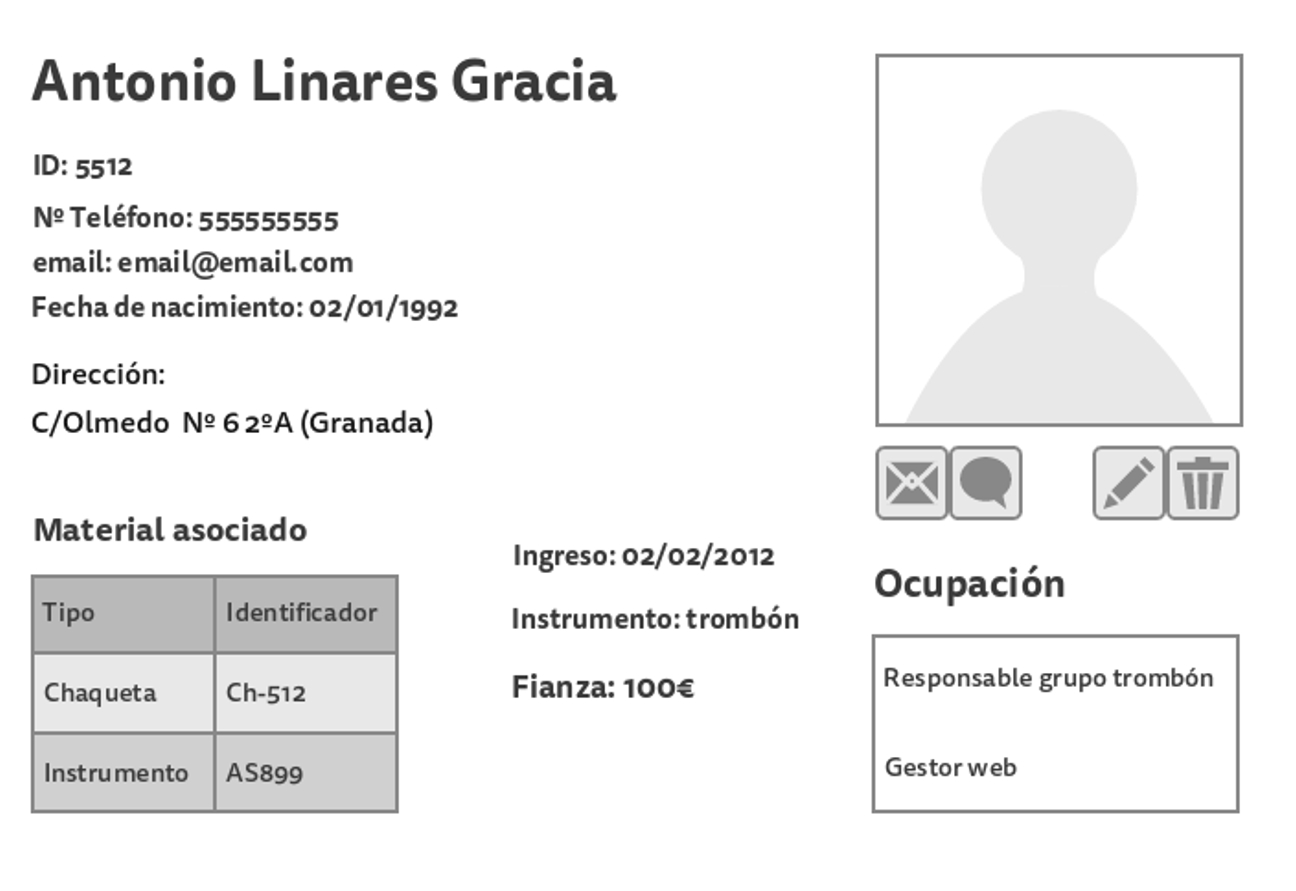
\includegraphics[width=0.75\textwidth]{img/patrimoniohumano.jpg}
\caption{Esquema sobre gestión de patrimonio musical}
\end{figure}

\subsubsection{Gestión de patrimonio físico}
Mediante la creación de un "catálogo" con todo el material del que dispone la banda,
se podrá saber cuándo es necesario renovarlo, la cantidad de material que hay sin utilizar
o quién tiene uno de esos materiales. Es decir, se tendrá una ficha donde se sepa:

\begin{itemize}
  \item Identificador
  \item Tipo
  \item Estado
  \item Fotografía
  \item Actual poseedor
\end{itemize}

\begin{figure}[!h]
\centering
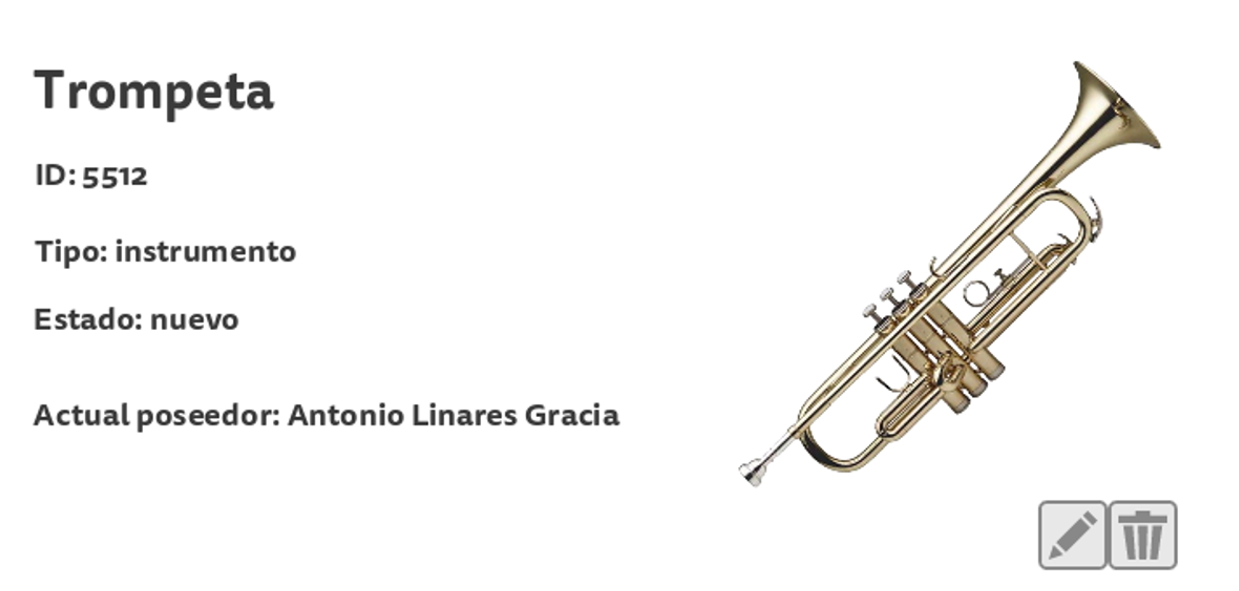
\includegraphics[width=0.75\textwidth]{img/patrimoniofisico.jpg}
\caption{Esquema sobre gestión de patrimonio musical}
\end{figure}

Además, para favorecer la rápida identificación de un material, se
dispondrá de un etiquetado como un código de barras o código QR.


\subsubsection{Gestión de patrimonio musical}
Uno de los problemas que se presentaban era la distribución de partituras entre los
músicos y el almacenamiento de las obras. En este sistema, se quiere facilitar a los
responsables estas tareas.\\
Un responsable de banda podrá subir las distintas partichelas y asignarlas a los
distintos músicos, de forma que puedan acceder a ellas cuando lo necesiten. Esto
permitirá, además, que los documentos se encuentren a salvo en la plataforma.

\begin{figure}[!h]
\centering
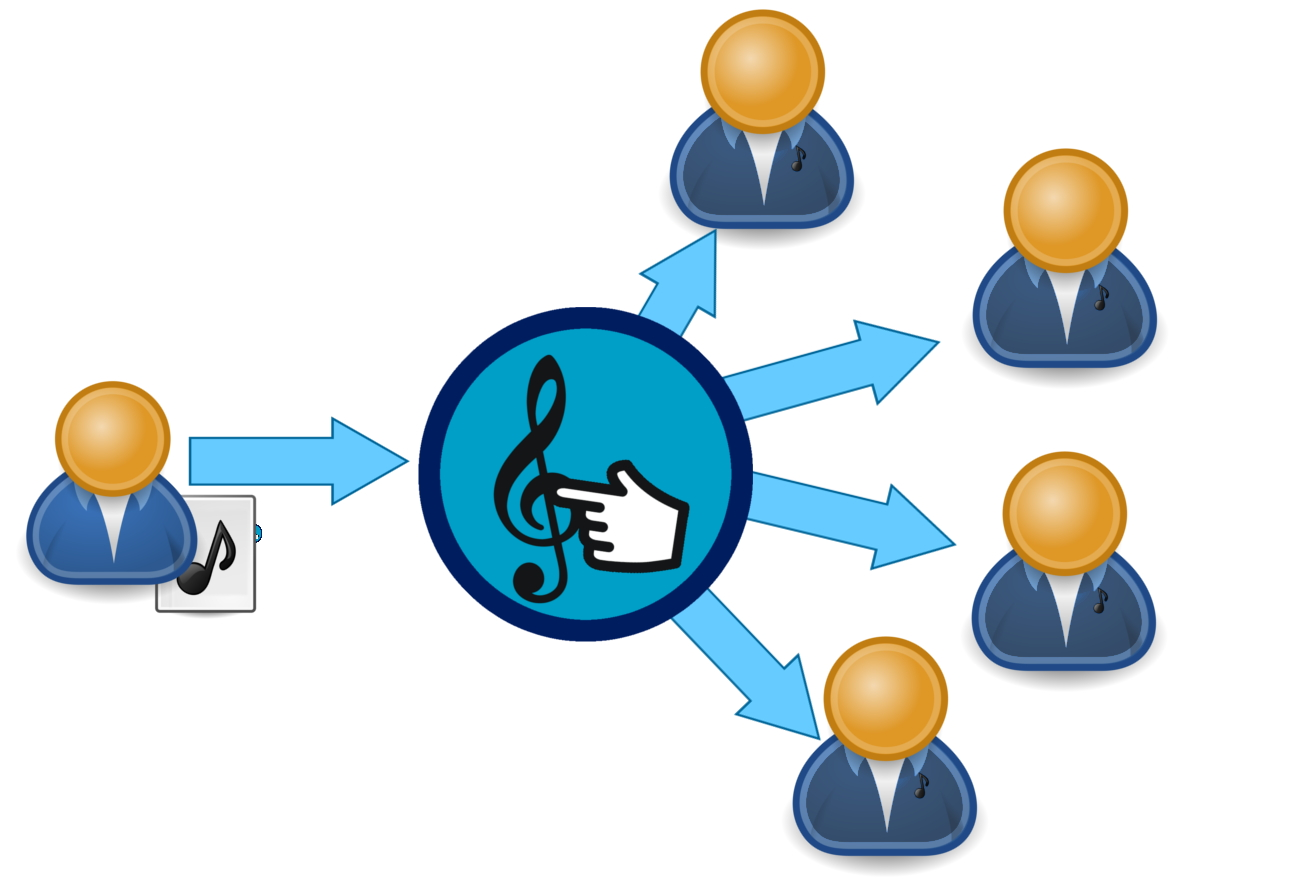
\includegraphics[width=0.5\textwidth]{img/patrimonio_musical.jpg}
\caption{Esquema sobre gestión de patrimonio musical}
\end{figure}

El sistema contará también con un catálogo común de partituras (de forma que un
responsable de banda pueda importar a su banda una composición).



\subsubsection{Comunicación entre junta/director/responsables y músicos}
Se quiere permitir que, aquellos usuarios que tengan los permisos necesarios,
puedan enviar mensajes de difusión a los distintos grupos de músicos (o a todos los
músicos de la banda) de la forma más sencilla posible.
\newline
Como se comentó en la breve descripción (\ref{breveDescripcion}), se tiene
planteado el desarrollo de una aplicación móvil para cada uno de los principales
sistemas operativos móviles (lo que permitirá que, tras enviarse un mensaje, todos
los usuarios lo reciban al instante). En caso que no exista aplicación para los sistemas
operativos móviles de


\end{document}
